\documentclass{jsarticle}
\usepackage[margin = .7in]{geometry}
\usepackage[dvipdfmx]{graphicx}
\usepackage{listings}
\usepackage{amsmath}
\usepackage{amsfonts}
\usepackage{bm}
\usepackage{ascmac}
\usepackage{MnSymbol}
\usepackage{multirow,array}
\usepackage{comment}
\lstset{%
  language={python},
  basicstyle={\small},%
  identifierstyle={\small},%
  commentstyle={\small\itshape},%
  keywordstyle={\small\bfseries},%
  ndkeywordstyle={\small},%
  stringstyle={\small\ttfamily},
  frame={tb},
  breaklines=true,
  columns=[l]{fullflexible},%
  numbers=left,%
  xrightmargin=0zw,%
  xleftmargin=3zw,%
  numberstyle={\scriptsize},%
  stepnumber=1,
  numbersep=1zw,%
  lineskip=-0.5ex%
}

\begin{document}
\title{ほげ}
\author{池上 慧}
\maketitle

\section{Introduction}
データの拡充と推定手法の開発、そしてそれを可能にする計算環境の実現に伴い戦略的状況を扱った実証分析は近年大きく進展している分野である。静学ゲームでは例えば\cite{1}で行われた寡占市場の分析や\cite{2},\cite{3},\cite{4}の参入の分析、\cite{5}による社会的相互作用モデルを用いたpeer effectの分析などが戦略的状況を扱った代表的な研究である。また動学ゲームにおいても、\cite{6}で開発された参入退出ゲームと\cite{9}や\cite{10}で開発された推定手法を用いて\cite{7}や\cite{8}などで動学的な要素を考慮した戦略的意思決定の実証が行われている。

こういった戦略的な状況の分析の基盤は現実のデータがある種の均衡状態から生み出されたものであるという構造を仮定することにある。静学ゲームでは完備情報下では純粋戦略ナッシュ均衡、不完備情報下であれば純粋戦略ベイジアンナッシュ均衡がプレイされているとしてモデルのパラメータを推定する。動学ゲームにおいても同様にマルコフ完全均衡がプレイされているという仮定の下でモデルのパラメータを推定する。

しかし現実にはモデルの予測するある種の均衡が必ずしもプレイされるわけではないということが実験を通して明らかにされてきた。そもそもナッシュ均衡の各種精緻化概念も現実をよりよく説明するために生み出されてきたものであるが、ホニャやホゲが提案した認知階層モデルやlevel-kモデルなどの限定合理性モデルも既存の均衡では予測できない実験データを説明するために作られたモデルである。こういったモデルの正当性は実験データをどれだけ説明できるかという基準で検証されるが、それはそのモデル自体の正当性ではなく、他のモデルと比しての妥当性に過ぎない。また、\cite{12}が指摘したようにデータへのフィットという観点でモデルの妥当性を図ることには正当性がない場合も存在する。

このようにモデルや均衡概念自体への検証というトピックは実験データを用いた場合にすら厳密な蓄積が少ないが、現実のデータを用いる場合にはほとんど研究の蓄積がない。\cite{13}はサッカーのペナルティキックにおける混合戦略ナッシュ均衡の実証を行い、\cite{11}はスウェーデンで実際に行われたゲームを用いて実験的状況下にないデータから均衡概念のチェックを行っている。こういった研究においても扱われる事象は極めて限定的かつ特殊なものであり、社会で広く観察される現象に対する均衡概念の検証はほとんど行われていない。この困難は研究者には観測できない変数の存在や異質性の問題、そしてそもそも利得が観測できずそれ自体が推定する対象であるパラメータであるという事実などによると考えられる。

本研究では広く観察される市場参入という現象に対して、戦略的状況の分析で一般に仮定される純粋戦略ナッシュ均衡を仮説検定によって検証する手法を提示する。モデルは\cite{2}で提案された完備情報参入ゲームを用いる。本論は以下のように進む。2章では関連する研究として\cite{11}と\cite{13}をレビューし、均衡に対する検証がなぜ困難かを整理する。3章では主要な結果を述べる。その際にモデルの説明、純粋戦略がとられていない場合の推定手法、純粋戦略ナッシュ均衡への検定という順番で進む。4章では結語としてより包括的な枠組みの可能性を述べる。


\section{Literatures}
段落1:levittのレビュー

段落2:Ostringのレビュー

\cite{11}で引用されているRobert Aumannの言葉にある通り、戦略的な状況を記述し分析するためにはそのゲームが厳格なルールを持っている必要がある。特に均衡を検証するという目的のためにはこれが重要であり、そのため利得をコントロールできる実験的状況や上記二つのような厳密なルールの下でプレイされるゲームしか検証に用いることができないのである。しかし一般に実証研究の対象となる経済事象はそのような理想的な状況ではなく、情報構造や利得の構造、さらに手番に関しても研究者にとっては不確実なものである。以下で扱う参入ゲームもその例外ではなく、実証に用いられるモデルは様々に特定化されている。

その特定化の一つとして純粋戦略ナッシュ均衡がプレイされているという仮定が置かれる。これは実現した結果についてプレイヤーが両者ともに別の行動をとればよかったと後悔することがないということを意味するが、支配戦略が存在しない事象においては強すぎる仮定である。よって、以下ではこの仮定を検証する枠組みを提示する。

\section{Results}
\subsection{Model}
以下の利得表を持つ参入ゲームを考える。
\begin{table}[h]
    \caption{利得表}
    \centering
    \setlength{\extrarowheight}{2pt}
    \begin{tabular}{cc|c|c|}
      & \multicolumn{1}{c}{} & \multicolumn{2}{c}{Player $2$}\\
      & \multicolumn{1}{c}{} & \multicolumn{1}{c}{参入しない}  & \multicolumn{1}{c}{参入する} \\\cline{3-4}
      \multirow{2}*{Player $1$}  & 参入しない & $(0,0)$ & $(0,\theta_{\mu}+\epsilon_2)$ \\\cline{3-4}
      & 参入する & $(\theta_{\mu}+\epsilon_1,0)$ & $(\theta_{\mu}+\theta_{\delta}+\epsilon_1, \theta_{\mu}+\theta_{\delta}+\epsilon_2)$ \\\cline{3-4}
    \end{tabular}
\end{table}
ここで、$\theta_{\mu}$は一社のみ参入することができた時に得られ利得であり、$\theta_{\delta}$は二社が参入してしまった時の利得減少分を表すパラメータである。$(\epsilon_1, \epsilon_2)$はプレイヤー同士では観測可能だが研究者には観測できない利得であり、標準正規分布に従うとする。この確率変数は各市場ごとに毎期生成される、つまりデータとして得られる市場ではそれぞれプレイヤーは異なる利得表のゲームをプレイしていることに注意する。以下「参入しない」を$0$、「参入する」を$1$で表記する。

プレイヤーは合理的であるとし、支配戦略がある時はその戦略をとることができるとする。例えばプレイヤー1については、
\begin{align*}
	\begin{cases}
		{\rm Pr}(\text{player 1 takes $0$}) = 1\quad \text{if}\ \epsilon_1 < -\theta_{\mu}\\
		{\rm Pr}(\text{player 1 takes $1$}) = 1\quad \text{if}\ \epsilon_1 > -\theta_{\mu} - \theta_{\delta}
	\end{cases}
\end{align*}
である。

また、支配戦略を用いて行動の逐次削除もできるとする。すなわち、相手にとって支配戦略が存在する時はその事実を用いて自身の行動について被支配戦略を削除することで行動を確定させることができる。例えばプレイヤー1について$-\theta_{\mu} < \epsilon_1 < -\theta_{\mu} - \theta_{\delta}$の時、
\begin{align*}
	\begin{cases}
		{\rm Pr}(\text{player 1 takes $0$}) = 1\quad \text{if}\ \epsilon_2 > -\theta_{\mu} - \theta_{\delta}\\
		{\rm Pr}(\text{player 1 takes $1$}) = 1\quad \text{if}\ \epsilon_2 < -\theta_{\mu}
	\end{cases}
\end{align*}
以上の仮定の下でプレイヤーの行動が確定しないのは$\left\{ (\epsilon_1, \epsilon_2) \mid -\theta_{\mu} < \epsilon_1 < -\theta_{\mu} - \theta_{\delta}\ \wedge\  -\theta_{\mu} < \epsilon_2 < -\theta_{\mu} - \theta_{\delta} \right\}$のみである。この領域(以下$\largestar$)における純粋戦略ナッシュ均衡は$(0,1),\ (1,0)$の二つである。

一方で$x$をプレイヤー1の参入しない確率、$y$をプレイヤー2の参入しない確率とした時に$(x, y) = \left( \frac{\theta_{\mu} + \theta_{\delta} + \nu_2}{\theta_{\delta}} ,  \frac{\theta_{\mu} + \theta_{\delta} + \nu_1}{\theta_{\delta}} \right)$が混合戦略ナッシュ均衡として存在する。$\largestar$において混合戦略がプレイされることは$(\epsilon_1, \epsilon_2) \in \largestar$でも一定の確率で$(1,1),\ (0,0)$が実現してしまうことを意味する。よって推定の際にはこの$(1,1),\ (0,0)$が実現する割合の歪みを適切に処理することが必要である。

\subsection{Inference}
\subsubsection{Bresnahan and Reissの推定手法}
純粋戦略を仮定した時、$\largestar$においては複数の均衡が存在するので単純にプレイヤーの参入結果を用いては適切な尤度を構成できない。しかし、$\largestar$において二つある純粋戦略ナッシュ均衡の結果がどちらも1社のみ参入するという結果であることを利用して、参入した企業の数を結果変数としたBivariate Probitを行うことでパラメータが推定できる。

$M$個の市場について企業の参入結果が得られているとする。$m_2$を2社がどちらも参入した市場の数、$m_1$を1社のみが参入した市場の数、$m_0$をどちらも参入しなかった市場の数として以下のように尤度が構成できる。
\begin{align*}
	L = \Phi(\theta_{\mu}+\theta_{\delta})^{m_2}\ \Phi(-\theta_{\mu})^{m_0}\  (1- \Phi(\theta_{\mu}+\theta_{\delta}) - \Phi(-\theta_{\mu}))^{m_1}
\end{align*}

\subsubsection{歪みの修正}
まず$\largestar$において混合戦略がプレイされているとした時に、$m_2$と$m_0$の中でどれだけが$\largestar$における混合戦略の結果として実現したものであるかを求める。

ベイズの定理より以下が成立する。ただし二つ目の等式は支配戦略はプレイされるという仮定より成立する。
\begin{align*}
	&{\rm Pr}(\text{(1,1) is NE}\ \mid\ \text{(1,1) is played}) \\[8pt]
	&= \frac{{\rm Pr}(\text{(1,1) is played}\ \mid\ \text{(1,1) is NE})\ {\rm Pr}(\text{(1,1) is NE})}{{\rm Pr}(\text{(1,1) is played}\ \mid\ \text{(1,1) is NE})\ {\rm Pr}(\text{(1,1) is NE}) + {\rm Pr}(\text{(1,1) is played}\ \mid\ \text{(1,1) is not NE})\ {\rm Pr}(\text{(1,1) is not NE})}\\[8pt]
	&= \frac{{\rm Pr}(\text{(1,1) is NE})}{{\rm Pr}(\text{(1,1) is NE}) + {\rm Pr}(\text{(1,1) is played}\ \mid\ \text{(1,1) is not NE})\ {\rm Pr}(\text{(1,1) is not NE})}\\[8pt]
	&= \frac{{\rm Pr}(\text{(1,1) is NE})}{{\rm Pr}(\text{(1,1) is NE}) + {\rm Pr}(\text{(1,1) is played} \wedge \largestar)}
\end{align*}
1社も参入しない場合についても同様の計算ができる。ここで${\rm Pr}(\text{(1,1) is NE}) = P_2(\theta_{\mu}, \theta_{\delta}),\ {\rm Pr}(\text{(0,0) is NE}) = P_0(\theta_{\mu}, \theta_{\delta})$と書くと、参入社数割合の修正式が以下のように得られる。

\begin{align*}
\begin{cases}
	f_1(\theta_{\mu}, \theta_{\delta}) = \frac{P_2(\theta_{\mu}, \theta_{\delta})}{P_2(\theta_{\mu}, \theta_{\delta}) + \iint_{\largestar} \frac{(\theta_{\mu}+\epsilon_1)(\theta_{\mu} + \epsilon_2)}{\theta_{\delta}^2} \phi_2(\epsilon_1, \epsilon_2) \mathrm{d}\epsilon_1 \mathrm{d}\epsilon_2}\\[30pt]
	f_2(\theta_{\mu}, \theta_{\delta}) = \frac{P_0(\theta_{\mu}, \theta_{\delta})}{P_0(\theta_{\mu}, \theta_{\delta}) + \iint_{\largestar} \left( 1 + \frac{\theta_{\mu} + \epsilon_1}{\theta_{\delta}} \right) \left( 1 + \frac{\theta_{\mu} + \epsilon_2}{\theta_{\delta}} \right) \phi_2(\epsilon_1, \epsilon_2) \mathrm{d}\epsilon_1 \mathrm{d}\epsilon_2}
\end{cases}
\end{align*}

これより推定においては以下の最大化問題を解けば良い。
\begin{align*}
	&\max_{\theta_{\mu}, \theta_{\delta}}\quad \Phi(\theta_{\mu}+\theta_{\delta})^{m_2^{*}}\ \Phi(-\theta_{\mu})^{m_0^{*}}\  (1- \Phi(\theta_{\mu}+\theta_{\delta}) - \Phi(-\theta_{\mu}))^{m_1^{*}}\\
	&\text{s.t.}\quad \begin{cases}
	m_2^{*} = f_1(\theta_{\mu}, \theta_{\delta})\ m_2\\
	m_0^{*} = f_2(\theta_{\mu}, \theta_{\delta})\ m_0\\
	m_1^{*} = M - m_2^{*} - m_0^{*}
	\end{cases}
\end{align*}
これは制約を代入すれば通常の最尤法と同じように推定できるが、微分が複雑となるため$(m_2^{*},m_0^{*},m_1^{*})$を逐次改定するアルゴリズムで推定する。$(\theta_{\mu}, \theta_{\delta}) = (1, -0.5)$を真の値とするときの収束の様子は図1のようになる。
\begin{figure}[h]
\centering
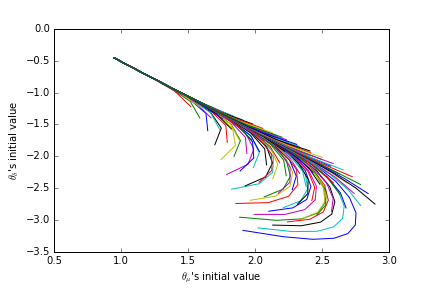
\includegraphics{conversion.png}
\caption{収束の様子}
\end{figure}

\subsection{Test}



\section{Conclusion}

\section{References}
\begin{thebibliography}{10}
	\bibitem{1} Bresnahan/寡占
	\bibitem{2} Bresnahan and Reiss
	\bibitem{3} Tamer 2003
	\bibitem{4} Seim 2006
	\bibitem{5} Brock and Durlauf
	\bibitem{6} Pakes and McGuire
	\bibitem{7} Collard and Wexler 2013
	\bibitem{8} Ryan 2012
	\bibitem{9} BBl 2007
	\bibitem{10} AM 2007
	\bibitem{11} Ostring et al 2011
	\bibitem{12} Haile 2008
	\bibitem{13} Levitt サッカー
	\bibitem{14} Eric van Damme 1998
\end{thebibliography}


\end{document}
























